\documentclass[twoside]{book}

% Packages required by doxygen
\usepackage{fixltx2e}
\usepackage{calc}
\usepackage{doxygen}
\usepackage[export]{adjustbox} % also loads graphicx
\usepackage{graphicx}
\usepackage[utf8]{inputenc}
\usepackage{makeidx}
\usepackage{multicol}
\usepackage{multirow}
\PassOptionsToPackage{warn}{textcomp}
\usepackage{textcomp}
\usepackage[nointegrals]{wasysym}
\usepackage[table]{xcolor}

% Font selection
\usepackage[T1]{fontenc}
\usepackage[scaled=.90]{helvet}
\usepackage{courier}
\usepackage{amssymb}
\usepackage{sectsty}
\renewcommand{\familydefault}{\sfdefault}
\allsectionsfont{%
  \fontseries{bc}\selectfont%
  \color{darkgray}%
}
\renewcommand{\DoxyLabelFont}{%
  \fontseries{bc}\selectfont%
  \color{darkgray}%
}
\newcommand{\+}{\discretionary{\mbox{\scriptsize$\hookleftarrow$}}{}{}}

% Page & text layout
\usepackage{geometry}
\geometry{%
  a4paper,%
  top=2.5cm,%
  bottom=2.5cm,%
  left=2.5cm,%
  right=2.5cm%
}
\tolerance=750
\hfuzz=15pt
\hbadness=750
\setlength{\emergencystretch}{15pt}
\setlength{\parindent}{0cm}
\setlength{\parskip}{0.2cm}
\makeatletter
\renewcommand{\paragraph}{%
  \@startsection{paragraph}{4}{0ex}{-1.0ex}{1.0ex}{%
    \normalfont\normalsize\bfseries\SS@parafont%
  }%
}
\renewcommand{\subparagraph}{%
  \@startsection{subparagraph}{5}{0ex}{-1.0ex}{1.0ex}{%
    \normalfont\normalsize\bfseries\SS@subparafont%
  }%
}
\makeatother

% Headers & footers
\usepackage{fancyhdr}
\pagestyle{fancyplain}
\fancyhead[LE]{\fancyplain{}{\bfseries\thepage}}
\fancyhead[CE]{\fancyplain{}{}}
\fancyhead[RE]{\fancyplain{}{\bfseries\leftmark}}
\fancyhead[LO]{\fancyplain{}{\bfseries\rightmark}}
\fancyhead[CO]{\fancyplain{}{}}
\fancyhead[RO]{\fancyplain{}{\bfseries\thepage}}
\fancyfoot[LE]{\fancyplain{}{}}
\fancyfoot[CE]{\fancyplain{}{}}
\fancyfoot[RE]{\fancyplain{}{\bfseries\scriptsize Generated on Fri Feb 20 2015 12\+:28\+:18 for Pyrst by Doxygen }}
\fancyfoot[LO]{\fancyplain{}{\bfseries\scriptsize Generated on Fri Feb 20 2015 12\+:28\+:18 for Pyrst by Doxygen }}
\fancyfoot[CO]{\fancyplain{}{}}
\fancyfoot[RO]{\fancyplain{}{}}
\renewcommand{\footrulewidth}{0.4pt}
\renewcommand{\chaptermark}[1]{%
  \markboth{#1}{}%
}
\renewcommand{\sectionmark}[1]{%
  \markright{\thesection\ #1}%
}

% Indices & bibliography
\usepackage{natbib}
\usepackage[titles]{tocloft}
\setcounter{tocdepth}{3}
\setcounter{secnumdepth}{5}
\makeindex

% Hyperlinks (required, but should be loaded last)
\usepackage{ifpdf}
\ifpdf
  \usepackage[pdftex,pagebackref=true]{hyperref}
\else
  \usepackage[ps2pdf,pagebackref=true]{hyperref}
\fi
\hypersetup{%
  colorlinks=true,%
  linkcolor=blue,%
  citecolor=blue,%
  unicode%
}

% Custom commands
\newcommand{\clearemptydoublepage}{%
  \newpage{\pagestyle{empty}\cleardoublepage}%
}


%===== C O N T E N T S =====

\begin{document}

% Titlepage & ToC
\hypersetup{pageanchor=false,
             bookmarks=true,
             bookmarksnumbered=true,
             pdfencoding=unicode
            }
\pagenumbering{roman}
\begin{titlepage}
\vspace*{7cm}
\begin{center}%
{\Large Pyrst \\[1ex]\large 0.\+50 }\\
\vspace*{1cm}
{\large Generated by Doxygen 1.8.9.1}\\
\vspace*{0.5cm}
{\small Fri Feb 20 2015 12:28:18}\\
\end{center}
\end{titlepage}
\clearemptydoublepage
\tableofcontents
\clearemptydoublepage
\pagenumbering{arabic}
\hypersetup{pageanchor=true}

%--- Begin generated contents ---
\chapter{Hierarchical Index}
\section{Class Hierarchy}
This inheritance list is sorted roughly, but not completely, alphabetically\+:\begin{DoxyCompactList}
\item Exception\begin{DoxyCompactList}
\item \contentsline{section}{pyrst.\+pyrst.\+exceptions.\+Auth\+Exception}{\pageref{classpyrst_1_1pyrst_1_1exceptions_1_1_auth_exception}}{}
\begin{DoxyCompactList}
\item \contentsline{section}{pyrst.\+pyrst.\+exceptions.\+Missing\+Credentials\+Exception}{\pageref{classpyrst_1_1pyrst_1_1exceptions_1_1_missing_credentials_exception}}{}
\item \contentsline{section}{pyrst.\+pyrst.\+exceptions.\+Missing\+Instance\+Exception}{\pageref{classpyrst_1_1pyrst_1_1exceptions_1_1_missing_instance_exception}}{}
\end{DoxyCompactList}
\item \contentsline{section}{pyrst.\+pyrst.\+exceptions.\+Connection\+Exception}{\pageref{classpyrst_1_1pyrst_1_1exceptions_1_1_connection_exception}}{}
\item \contentsline{section}{pyrst.\+pyrst.\+exceptions.\+Space\+I\+D\+Exception}{\pageref{classpyrst_1_1pyrst_1_1exceptions_1_1_space_i_d_exception}}{}
\item \contentsline{section}{pyrst.\+pyrst.\+exceptions.\+Token\+Exception}{\pageref{classpyrst_1_1pyrst_1_1exceptions_1_1_token_exception}}{}
\end{DoxyCompactList}
\item object\begin{DoxyCompactList}
\item \contentsline{section}{pyrst.\+pyrst.\+client.\+Birst\+Client}{\pageref{classpyrst_1_1pyrst_1_1client_1_1_birst_client}}{}
\item \contentsline{section}{pyrst.\+pyrst.\+handlers.\+Handler}{\pageref{classpyrst_1_1pyrst_1_1handlers_1_1_handler}}{}
\begin{DoxyCompactList}
\item \contentsline{section}{pyrst.\+pyrst.\+handlers.\+Df\+Handler}{\pageref{classpyrst_1_1pyrst_1_1handlers_1_1_df_handler}}{}
\end{DoxyCompactList}
\item \contentsline{section}{pyrst.\+pyrst.\+helpers.\+Instance}{\pageref{classpyrst_1_1pyrst_1_1helpers_1_1_instance}}{}
\end{DoxyCompactList}
\end{DoxyCompactList}

\chapter{Class Index}
\section{Class List}
Here are the classes, structs, unions and interfaces with brief descriptions\+:\begin{DoxyCompactList}
\item\contentsline{section}{\hyperlink{classpyrst_1_1pyrst_1_1exceptions_1_1_auth_exception}{pyrst.\+pyrst.\+exceptions.\+Auth\+Exception} }{\pageref{classpyrst_1_1pyrst_1_1exceptions_1_1_auth_exception}}{}
\item\contentsline{section}{\hyperlink{classpyrst_1_1pyrst_1_1client_1_1_birst_client}{pyrst.\+pyrst.\+client.\+Birst\+Client} }{\pageref{classpyrst_1_1pyrst_1_1client_1_1_birst_client}}{}
\item\contentsline{section}{\hyperlink{classpyrst_1_1pyrst_1_1exceptions_1_1_connection_exception}{pyrst.\+pyrst.\+exceptions.\+Connection\+Exception} }{\pageref{classpyrst_1_1pyrst_1_1exceptions_1_1_connection_exception}}{}
\item\contentsline{section}{\hyperlink{classpyrst_1_1pyrst_1_1handlers_1_1_df_handler}{pyrst.\+pyrst.\+handlers.\+Df\+Handler} }{\pageref{classpyrst_1_1pyrst_1_1handlers_1_1_df_handler}}{}
\item\contentsline{section}{\hyperlink{classpyrst_1_1pyrst_1_1handlers_1_1_handler}{pyrst.\+pyrst.\+handlers.\+Handler} }{\pageref{classpyrst_1_1pyrst_1_1handlers_1_1_handler}}{}
\item\contentsline{section}{\hyperlink{classpyrst_1_1pyrst_1_1helpers_1_1_instance}{pyrst.\+pyrst.\+helpers.\+Instance} }{\pageref{classpyrst_1_1pyrst_1_1helpers_1_1_instance}}{}
\item\contentsline{section}{\hyperlink{classpyrst_1_1pyrst_1_1exceptions_1_1_missing_credentials_exception}{pyrst.\+pyrst.\+exceptions.\+Missing\+Credentials\+Exception} }{\pageref{classpyrst_1_1pyrst_1_1exceptions_1_1_missing_credentials_exception}}{}
\item\contentsline{section}{\hyperlink{classpyrst_1_1pyrst_1_1exceptions_1_1_missing_instance_exception}{pyrst.\+pyrst.\+exceptions.\+Missing\+Instance\+Exception} }{\pageref{classpyrst_1_1pyrst_1_1exceptions_1_1_missing_instance_exception}}{}
\item\contentsline{section}{\hyperlink{classpyrst_1_1pyrst_1_1exceptions_1_1_space_i_d_exception}{pyrst.\+pyrst.\+exceptions.\+Space\+I\+D\+Exception} }{\pageref{classpyrst_1_1pyrst_1_1exceptions_1_1_space_i_d_exception}}{}
\item\contentsline{section}{\hyperlink{classpyrst_1_1pyrst_1_1exceptions_1_1_token_exception}{pyrst.\+pyrst.\+exceptions.\+Token\+Exception} }{\pageref{classpyrst_1_1pyrst_1_1exceptions_1_1_token_exception}}{}
\end{DoxyCompactList}

\chapter{Class Documentation}
\hypertarget{classpyrst_1_1pyrst_1_1exceptions_1_1_auth_exception}{}\section{pyrst.\+pyrst.\+exceptions.\+Auth\+Exception Class Reference}
\label{classpyrst_1_1pyrst_1_1exceptions_1_1_auth_exception}\index{pyrst.\+pyrst.\+exceptions.\+Auth\+Exception@{pyrst.\+pyrst.\+exceptions.\+Auth\+Exception}}
Inheritance diagram for pyrst.\+pyrst.\+exceptions.\+Auth\+Exception\+:\begin{figure}[H]
\begin{center}
\leavevmode
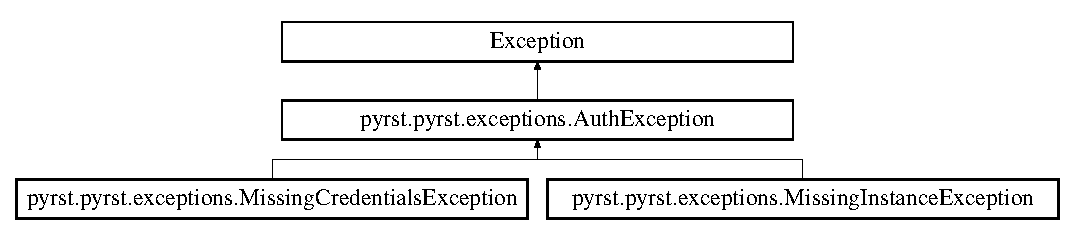
\includegraphics[height=2.709677cm]{classpyrst_1_1pyrst_1_1exceptions_1_1_auth_exception}
\end{center}
\end{figure}
\subsection*{Public Member Functions}
\begin{DoxyCompactItemize}
\item 
\hypertarget{classpyrst_1_1pyrst_1_1exceptions_1_1_auth_exception_a60275b6315178b392e46755c9e38246e}{}def {\bfseries \+\_\+\+\_\+repr\+\_\+\+\_\+} (self)\label{classpyrst_1_1pyrst_1_1exceptions_1_1_auth_exception_a60275b6315178b392e46755c9e38246e}

\end{DoxyCompactItemize}


The documentation for this class was generated from the following file\+:\begin{DoxyCompactItemize}
\item 
pyrst/exceptions.\+py\end{DoxyCompactItemize}

\hypertarget{classpyrst_1_1pyrst_1_1client_1_1_birst_client}{}\section{pyrst.\+pyrst.\+client.\+Birst\+Client Class Reference}
\label{classpyrst_1_1pyrst_1_1client_1_1_birst_client}\index{pyrst.\+pyrst.\+client.\+Birst\+Client@{pyrst.\+pyrst.\+client.\+Birst\+Client}}
Inheritance diagram for pyrst.\+pyrst.\+client.\+Birst\+Client\+:\begin{figure}[H]
\begin{center}
\leavevmode
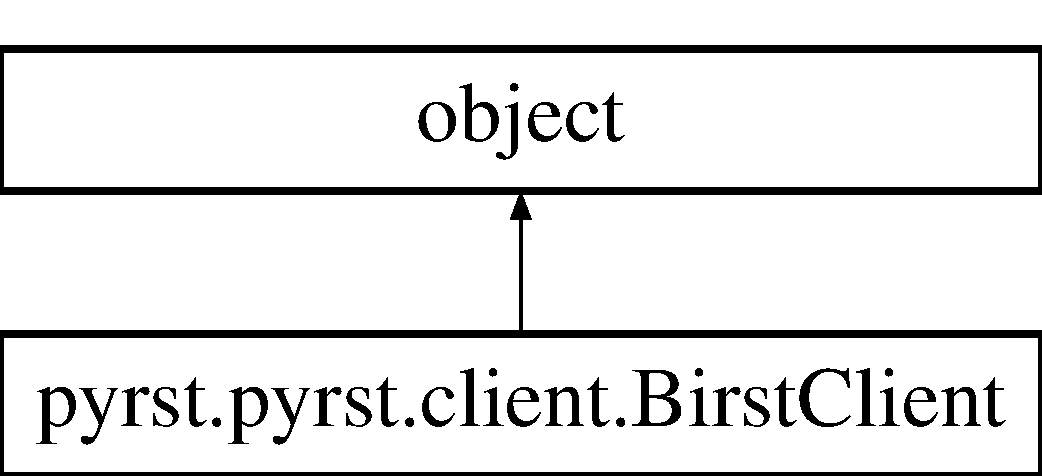
\includegraphics[height=2.000000cm]{classpyrst_1_1pyrst_1_1client_1_1_birst_client}
\end{center}
\end{figure}
\subsection*{Public Member Functions}
\begin{DoxyCompactItemize}
\item 
\hypertarget{classpyrst_1_1pyrst_1_1client_1_1_birst_client_a2d349d2e5f467a367a07de6dad164269}{}def {\bfseries \+\_\+\+\_\+init\+\_\+\+\_\+}\label{classpyrst_1_1pyrst_1_1client_1_1_birst_client_a2d349d2e5f467a367a07de6dad164269}

\item 
\hypertarget{classpyrst_1_1pyrst_1_1client_1_1_birst_client_aa367e96d5a65ce5d4afd9a0bd25c2889}{}def {\bfseries \+\_\+\+\_\+repr\+\_\+\+\_\+} (self)\label{classpyrst_1_1pyrst_1_1client_1_1_birst_client_aa367e96d5a65ce5d4afd9a0bd25c2889}

\item 
def \hyperlink{classpyrst_1_1pyrst_1_1client_1_1_birst_client_ab0090c1a32abe9f701063ba814d23656}{login} (self)
\begin{DoxyCompactList}\small\item\em L\+O\+G\+I\+N A\+N\+D L\+O\+G\+O\+U\+T \#. \end{DoxyCompactList}\item 
def \hyperlink{classpyrst_1_1pyrst_1_1client_1_1_birst_client_a92c654912a5a6e0e4590fa1714463956}{logout} (self)
\item 
def \hyperlink{classpyrst_1_1pyrst_1_1client_1_1_birst_client_a5420fea6cda5cee1115a376e1e24115d}{executequery}
\begin{DoxyCompactList}\small\item\em Q\+U\+E\+R\+Y\+I\+N\+G \#. \end{DoxyCompactList}\item 
def \hyperlink{classpyrst_1_1pyrst_1_1client_1_1_birst_client_ae346cadad3a8cf2b479c572a1da846d4}{retrieve}
\end{DoxyCompactItemize}
\subsection*{Public Attributes}
\begin{DoxyCompactItemize}
\item 
\hypertarget{classpyrst_1_1pyrst_1_1client_1_1_birst_client_a9efbb932ee5e4ef4158da2a34fb748b5}{}{\bfseries password}\label{classpyrst_1_1pyrst_1_1client_1_1_birst_client_a9efbb932ee5e4ef4158da2a34fb748b5}

\item 
\hypertarget{classpyrst_1_1pyrst_1_1client_1_1_birst_client_aa6b17ebf4b4f24fe48510bbe4d576f1b}{}{\bfseries user}\label{classpyrst_1_1pyrst_1_1client_1_1_birst_client_aa6b17ebf4b4f24fe48510bbe4d576f1b}

\item 
\hypertarget{classpyrst_1_1pyrst_1_1client_1_1_birst_client_abdfde1fd8dd0c8ea85269c0c25e24b90}{}{\bfseries instance}\label{classpyrst_1_1pyrst_1_1client_1_1_birst_client_abdfde1fd8dd0c8ea85269c0c25e24b90}

\item 
\hypertarget{classpyrst_1_1pyrst_1_1client_1_1_birst_client_a3444c0f48bff8492fbfa22c939530a94}{}{\bfseries token}\label{classpyrst_1_1pyrst_1_1client_1_1_birst_client_a3444c0f48bff8492fbfa22c939530a94}

\item 
\hypertarget{classpyrst_1_1pyrst_1_1client_1_1_birst_client_a3bb07a58d56486da55c7ca3bb3741cfd}{}{\bfseries connector}\label{classpyrst_1_1pyrst_1_1client_1_1_birst_client_a3bb07a58d56486da55c7ca3bb3741cfd}

\end{DoxyCompactItemize}


\subsection{Detailed Description}
\begin{DoxyVerb}Basic Birst client object.
\end{DoxyVerb}
 

\subsection{Member Function Documentation}
\hypertarget{classpyrst_1_1pyrst_1_1client_1_1_birst_client_a5420fea6cda5cee1115a376e1e24115d}{}\index{pyrst\+::pyrst\+::client\+::\+Birst\+Client@{pyrst\+::pyrst\+::client\+::\+Birst\+Client}!executequery@{executequery}}
\index{executequery@{executequery}!pyrst\+::pyrst\+::client\+::\+Birst\+Client@{pyrst\+::pyrst\+::client\+::\+Birst\+Client}}
\subsubsection[{executequery}]{\setlength{\rightskip}{0pt plus 5cm}def pyrst.\+pyrst.\+client.\+Birst\+Client.\+executequery (
\begin{DoxyParamCaption}
\item[{}]{self, }
\item[{}]{space, }
\item[{}]{query, }
\item[{}]{handler = {\ttfamily None}}
\end{DoxyParamCaption}
)}\label{classpyrst_1_1pyrst_1_1client_1_1_birst_client_a5420fea6cda5cee1115a376e1e24115d}


Q\+U\+E\+R\+Y\+I\+N\+G \#. 

The query interface exposes three methods\+:
\begin{DoxyItemize}
\item executequery\+: simple querying
\item more\+: continue querying
\item retrieve\+: keep querying as long as there are results.
\end{DoxyItemize}

Unlike in Birst\textquotesingle{}s X\+M\+L A\+P\+I, in Pyrst, the space comes {\itshape before} the query -\/ this is much more intuitive since the query is subordinate to the space rather than the other way around. \begin{DoxyVerb}Retrieves the first 1,000 results for the query.

:param space: SpaceID of the space (incl. hyphens, 36 chars)
:param query: Birst BQL query
:param handler: instance of output handler class
:return: query result
\end{DoxyVerb}
 \hypertarget{classpyrst_1_1pyrst_1_1client_1_1_birst_client_ab0090c1a32abe9f701063ba814d23656}{}\index{pyrst\+::pyrst\+::client\+::\+Birst\+Client@{pyrst\+::pyrst\+::client\+::\+Birst\+Client}!login@{login}}
\index{login@{login}!pyrst\+::pyrst\+::client\+::\+Birst\+Client@{pyrst\+::pyrst\+::client\+::\+Birst\+Client}}
\subsubsection[{login}]{\setlength{\rightskip}{0pt plus 5cm}def pyrst.\+pyrst.\+client.\+Birst\+Client.\+login (
\begin{DoxyParamCaption}
\item[{}]{self}
\end{DoxyParamCaption}
)}\label{classpyrst_1_1pyrst_1_1client_1_1_birst_client_ab0090c1a32abe9f701063ba814d23656}


L\+O\+G\+I\+N A\+N\+D L\+O\+G\+O\+U\+T \#. 

The login A\+P\+I exposes two (fairly selfexplanatory) methods\+:
\begin{DoxyItemize}
\item login
\item logout
\end{DoxyItemize}

There is no manual token handling in Pyrst -\/ upon login, your token will be appended to the instance as an instance variable. \begin{DoxyVerb}Logs the user in to the instance specified in the basic settings of the
class with the password and username specified.
If successful, the token returned will be appended to the class instance
as an instance variable.
\end{DoxyVerb}
 \hypertarget{classpyrst_1_1pyrst_1_1client_1_1_birst_client_a92c654912a5a6e0e4590fa1714463956}{}\index{pyrst\+::pyrst\+::client\+::\+Birst\+Client@{pyrst\+::pyrst\+::client\+::\+Birst\+Client}!logout@{logout}}
\index{logout@{logout}!pyrst\+::pyrst\+::client\+::\+Birst\+Client@{pyrst\+::pyrst\+::client\+::\+Birst\+Client}}
\subsubsection[{logout}]{\setlength{\rightskip}{0pt plus 5cm}def pyrst.\+pyrst.\+client.\+Birst\+Client.\+logout (
\begin{DoxyParamCaption}
\item[{}]{self}
\end{DoxyParamCaption}
)}\label{classpyrst_1_1pyrst_1_1client_1_1_birst_client_a92c654912a5a6e0e4590fa1714463956}
\begin{DoxyVerb}Logs the user out and deletes the token saved in the instance.
\end{DoxyVerb}
 \hypertarget{classpyrst_1_1pyrst_1_1client_1_1_birst_client_ae346cadad3a8cf2b479c572a1da846d4}{}\index{pyrst\+::pyrst\+::client\+::\+Birst\+Client@{pyrst\+::pyrst\+::client\+::\+Birst\+Client}!retrieve@{retrieve}}
\index{retrieve@{retrieve}!pyrst\+::pyrst\+::client\+::\+Birst\+Client@{pyrst\+::pyrst\+::client\+::\+Birst\+Client}}
\subsubsection[{retrieve}]{\setlength{\rightskip}{0pt plus 5cm}def pyrst.\+pyrst.\+client.\+Birst\+Client.\+retrieve (
\begin{DoxyParamCaption}
\item[{}]{self, }
\item[{}]{space, }
\item[{}]{query, }
\item[{}]{handler = {\ttfamily None}}
\end{DoxyParamCaption}
)}\label{classpyrst_1_1pyrst_1_1client_1_1_birst_client_ae346cadad3a8cf2b479c572a1da846d4}
\begin{DoxyVerb}Retrieves the entire dataset for the query.

:param space: SpaceID of the space (incl. hyphens, 36 chars)
:param query: Birst BQL query
:param handler: instance of output handler class
:return: query result
\end{DoxyVerb}
 

The documentation for this class was generated from the following file\+:\begin{DoxyCompactItemize}
\item 
pyrst/client.\+py\end{DoxyCompactItemize}

\hypertarget{classpyrst_1_1pyrst_1_1exceptions_1_1_connection_exception}{}\section{pyrst.\+pyrst.\+exceptions.\+Connection\+Exception Class Reference}
\label{classpyrst_1_1pyrst_1_1exceptions_1_1_connection_exception}\index{pyrst.\+pyrst.\+exceptions.\+Connection\+Exception@{pyrst.\+pyrst.\+exceptions.\+Connection\+Exception}}
Inheritance diagram for pyrst.\+pyrst.\+exceptions.\+Connection\+Exception\+:\begin{figure}[H]
\begin{center}
\leavevmode
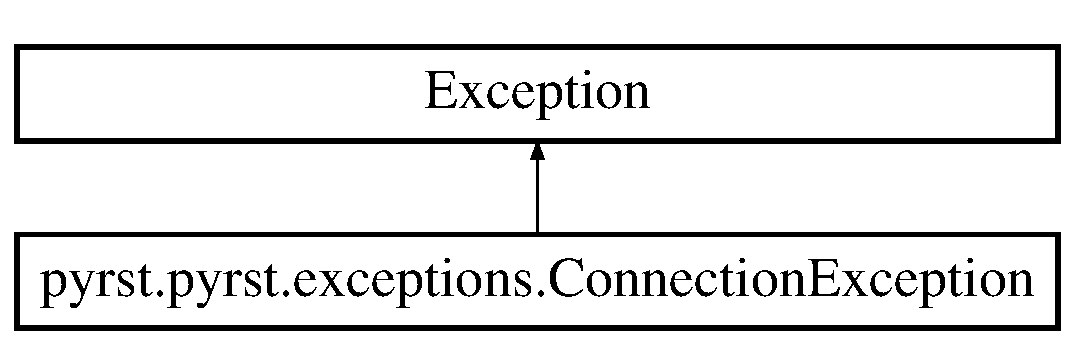
\includegraphics[height=2.000000cm]{classpyrst_1_1pyrst_1_1exceptions_1_1_connection_exception}
\end{center}
\end{figure}
\subsection*{Public Member Functions}
\begin{DoxyCompactItemize}
\item 
\hypertarget{classpyrst_1_1pyrst_1_1exceptions_1_1_connection_exception_a656fe7d3628524a52c21291116affe1a}{}def {\bfseries \+\_\+\+\_\+repr\+\_\+\+\_\+} (self)\label{classpyrst_1_1pyrst_1_1exceptions_1_1_connection_exception_a656fe7d3628524a52c21291116affe1a}

\end{DoxyCompactItemize}


The documentation for this class was generated from the following file\+:\begin{DoxyCompactItemize}
\item 
pyrst/exceptions.\+py\end{DoxyCompactItemize}

\hypertarget{classpyrst_1_1pyrst_1_1handlers_1_1_df_handler}{}\section{pyrst.\+pyrst.\+handlers.\+Df\+Handler Class Reference}
\label{classpyrst_1_1pyrst_1_1handlers_1_1_df_handler}\index{pyrst.\+pyrst.\+handlers.\+Df\+Handler@{pyrst.\+pyrst.\+handlers.\+Df\+Handler}}
Inheritance diagram for pyrst.\+pyrst.\+handlers.\+Df\+Handler\+:\begin{figure}[H]
\begin{center}
\leavevmode
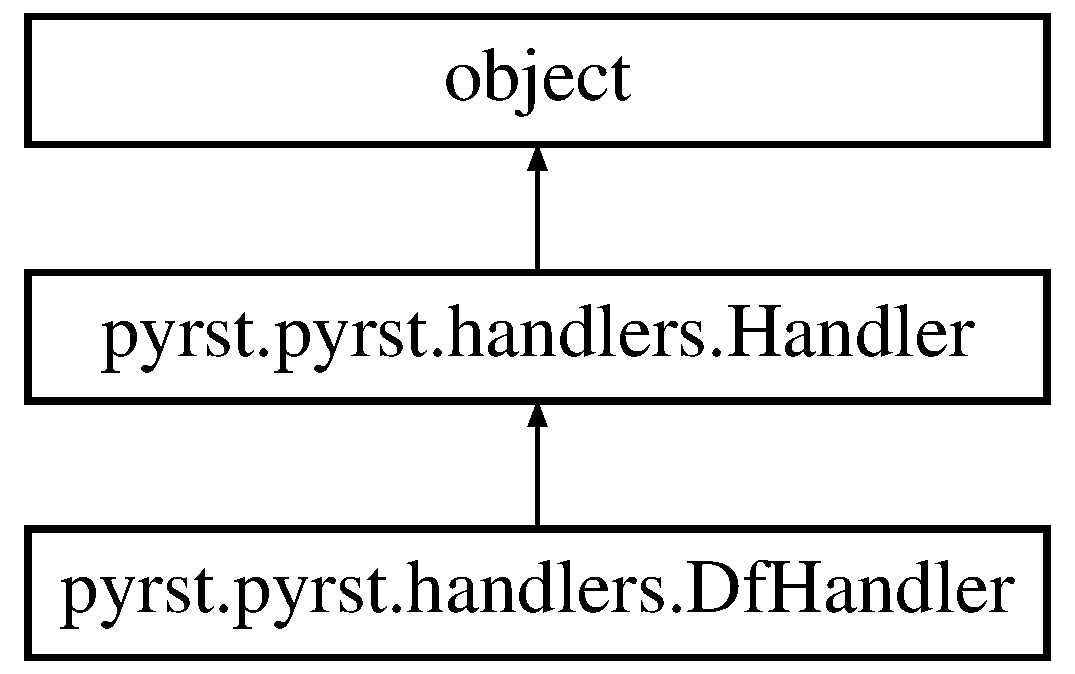
\includegraphics[height=3.000000cm]{classpyrst_1_1pyrst_1_1handlers_1_1_df_handler}
\end{center}
\end{figure}
\subsection*{Public Member Functions}
\begin{DoxyCompactItemize}
\item 
\hypertarget{classpyrst_1_1pyrst_1_1handlers_1_1_df_handler_a0121c1c288ebc45a0f4c4499c72dd5b4}{}def {\bfseries process} (self, query\+\_\+output)\label{classpyrst_1_1pyrst_1_1handlers_1_1_df_handler_a0121c1c288ebc45a0f4c4499c72dd5b4}

\end{DoxyCompactItemize}


\subsection{Detailed Description}
\begin{DoxyVerb}Handler that returns a Pandas dataFrame
\end{DoxyVerb}
 

The documentation for this class was generated from the following file\+:\begin{DoxyCompactItemize}
\item 
pyrst/handlers.\+py\end{DoxyCompactItemize}

\hypertarget{classpyrst_1_1pyrst_1_1handlers_1_1_handler}{}\section{pyrst.\+pyrst.\+handlers.\+Handler Class Reference}
\label{classpyrst_1_1pyrst_1_1handlers_1_1_handler}\index{pyrst.\+pyrst.\+handlers.\+Handler@{pyrst.\+pyrst.\+handlers.\+Handler}}
Inheritance diagram for pyrst.\+pyrst.\+handlers.\+Handler\+:\begin{figure}[H]
\begin{center}
\leavevmode
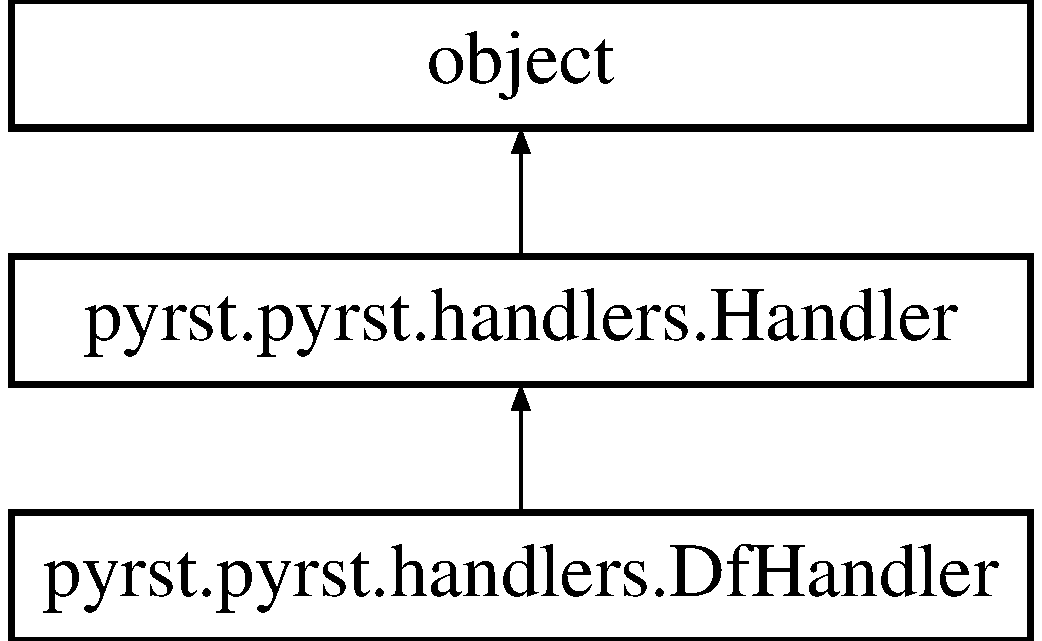
\includegraphics[height=3.000000cm]{classpyrst_1_1pyrst_1_1handlers_1_1_handler}
\end{center}
\end{figure}
\subsection*{Public Member Functions}
\begin{DoxyCompactItemize}
\item 
\hypertarget{classpyrst_1_1pyrst_1_1handlers_1_1_handler_a15f25cdd5267f1bc9aef3669863b5c8e}{}def {\bfseries \+\_\+\+\_\+repr\+\_\+\+\_\+} (self)\label{classpyrst_1_1pyrst_1_1handlers_1_1_handler_a15f25cdd5267f1bc9aef3669863b5c8e}

\item 
\hypertarget{classpyrst_1_1pyrst_1_1handlers_1_1_handler_acbe028926c19f7228c02ef405e27825b}{}def {\bfseries process} (self, query\+\_\+output)\label{classpyrst_1_1pyrst_1_1handlers_1_1_handler_acbe028926c19f7228c02ef405e27825b}

\end{DoxyCompactItemize}


The documentation for this class was generated from the following file\+:\begin{DoxyCompactItemize}
\item 
pyrst/handlers.\+py\end{DoxyCompactItemize}

\hypertarget{classpyrst_1_1pyrst_1_1helpers_1_1_instance}{}\section{pyrst.\+pyrst.\+helpers.\+Instance Class Reference}
\label{classpyrst_1_1pyrst_1_1helpers_1_1_instance}\index{pyrst.\+pyrst.\+helpers.\+Instance@{pyrst.\+pyrst.\+helpers.\+Instance}}
Inheritance diagram for pyrst.\+pyrst.\+helpers.\+Instance\+:\begin{figure}[H]
\begin{center}
\leavevmode
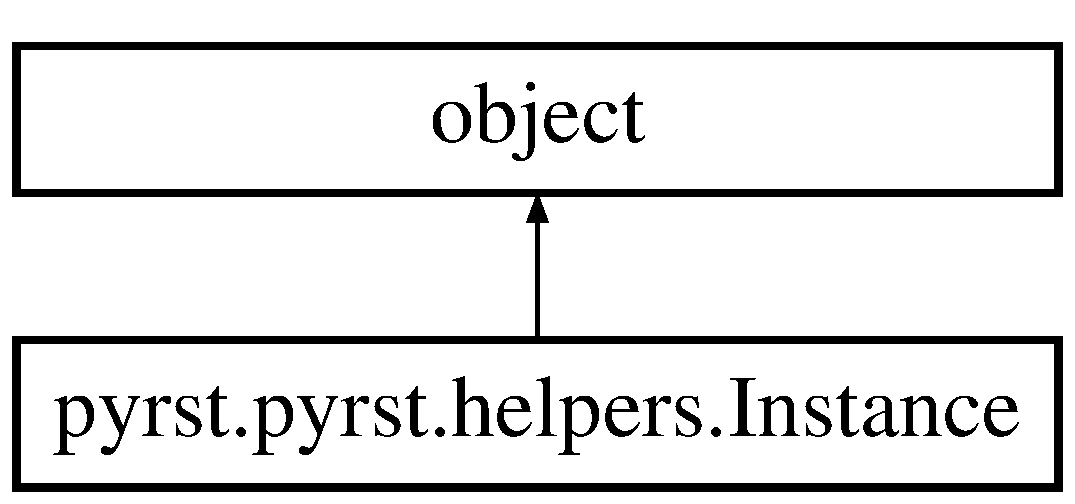
\includegraphics[height=2.000000cm]{classpyrst_1_1pyrst_1_1helpers_1_1_instance}
\end{center}
\end{figure}
\subsection*{Public Member Functions}
\begin{DoxyCompactItemize}
\item 
\hypertarget{classpyrst_1_1pyrst_1_1helpers_1_1_instance_abbfff8f9320f6f52629a32cc796538f7}{}def {\bfseries \+\_\+\+\_\+init\+\_\+\+\_\+} (self, colnames, rows)\label{classpyrst_1_1pyrst_1_1helpers_1_1_instance_abbfff8f9320f6f52629a32cc796538f7}

\end{DoxyCompactItemize}
\subsection*{Public Attributes}
\begin{DoxyCompactItemize}
\item 
\hypertarget{classpyrst_1_1pyrst_1_1helpers_1_1_instance_af4a45c81b48048340c6ae19f8899ca9e}{}{\bfseries colnames}\label{classpyrst_1_1pyrst_1_1helpers_1_1_instance_af4a45c81b48048340c6ae19f8899ca9e}

\item 
\hypertarget{classpyrst_1_1pyrst_1_1helpers_1_1_instance_aba9410bbd256503becd58fc393cc08f2}{}{\bfseries rows}\label{classpyrst_1_1pyrst_1_1helpers_1_1_instance_aba9410bbd256503becd58fc393cc08f2}

\end{DoxyCompactItemize}


The documentation for this class was generated from the following file\+:\begin{DoxyCompactItemize}
\item 
pyrst/helpers.\+py\end{DoxyCompactItemize}

\hypertarget{classpyrst_1_1pyrst_1_1exceptions_1_1_missing_credentials_exception}{}\section{pyrst.\+pyrst.\+exceptions.\+Missing\+Credentials\+Exception Class Reference}
\label{classpyrst_1_1pyrst_1_1exceptions_1_1_missing_credentials_exception}\index{pyrst.\+pyrst.\+exceptions.\+Missing\+Credentials\+Exception@{pyrst.\+pyrst.\+exceptions.\+Missing\+Credentials\+Exception}}
Inheritance diagram for pyrst.\+pyrst.\+exceptions.\+Missing\+Credentials\+Exception\+:\begin{figure}[H]
\begin{center}
\leavevmode
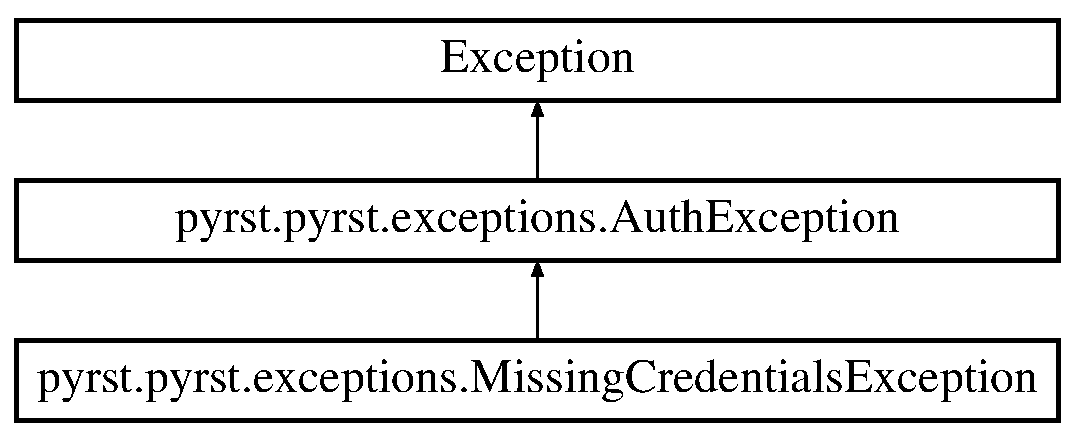
\includegraphics[height=3.000000cm]{classpyrst_1_1pyrst_1_1exceptions_1_1_missing_credentials_exception}
\end{center}
\end{figure}
\subsection*{Public Member Functions}
\begin{DoxyCompactItemize}
\item 
\hypertarget{classpyrst_1_1pyrst_1_1exceptions_1_1_missing_credentials_exception_a532736b9cb49859c7c8a3dab5f6b8cdc}{}def {\bfseries \+\_\+\+\_\+repr\+\_\+\+\_\+} (self)\label{classpyrst_1_1pyrst_1_1exceptions_1_1_missing_credentials_exception_a532736b9cb49859c7c8a3dab5f6b8cdc}

\end{DoxyCompactItemize}


The documentation for this class was generated from the following file\+:\begin{DoxyCompactItemize}
\item 
pyrst/exceptions.\+py\end{DoxyCompactItemize}

\hypertarget{classpyrst_1_1pyrst_1_1exceptions_1_1_missing_instance_exception}{}\section{pyrst.\+pyrst.\+exceptions.\+Missing\+Instance\+Exception Class Reference}
\label{classpyrst_1_1pyrst_1_1exceptions_1_1_missing_instance_exception}\index{pyrst.\+pyrst.\+exceptions.\+Missing\+Instance\+Exception@{pyrst.\+pyrst.\+exceptions.\+Missing\+Instance\+Exception}}
Inheritance diagram for pyrst.\+pyrst.\+exceptions.\+Missing\+Instance\+Exception\+:\begin{figure}[H]
\begin{center}
\leavevmode
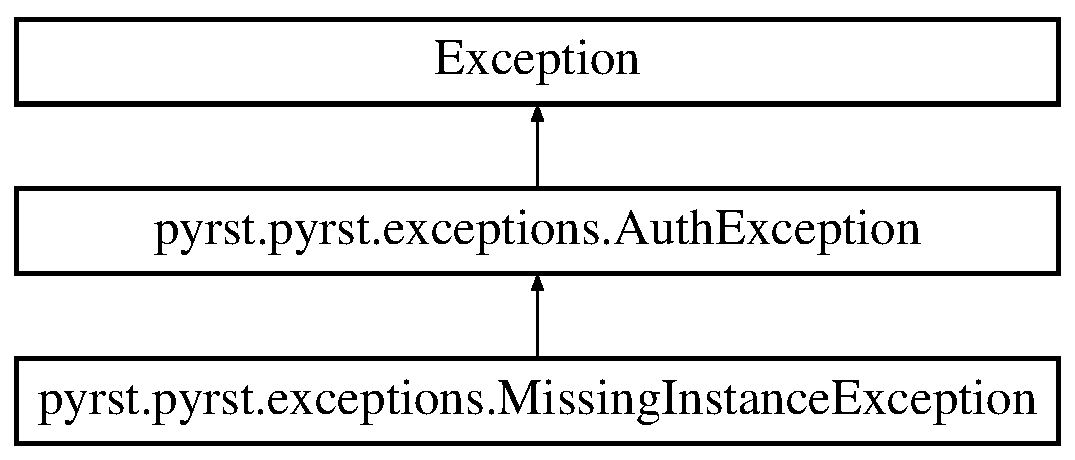
\includegraphics[height=3.000000cm]{classpyrst_1_1pyrst_1_1exceptions_1_1_missing_instance_exception}
\end{center}
\end{figure}
\subsection*{Public Member Functions}
\begin{DoxyCompactItemize}
\item 
\hypertarget{classpyrst_1_1pyrst_1_1exceptions_1_1_missing_instance_exception_aae1a4694bead8963b736aef0c884fd90}{}def {\bfseries \+\_\+\+\_\+repr\+\_\+\+\_\+} (self)\label{classpyrst_1_1pyrst_1_1exceptions_1_1_missing_instance_exception_aae1a4694bead8963b736aef0c884fd90}

\end{DoxyCompactItemize}


The documentation for this class was generated from the following file\+:\begin{DoxyCompactItemize}
\item 
pyrst/exceptions.\+py\end{DoxyCompactItemize}

\hypertarget{classpyrst_1_1pyrst_1_1exceptions_1_1_space_i_d_exception}{}\section{pyrst.\+pyrst.\+exceptions.\+Space\+I\+D\+Exception Class Reference}
\label{classpyrst_1_1pyrst_1_1exceptions_1_1_space_i_d_exception}\index{pyrst.\+pyrst.\+exceptions.\+Space\+I\+D\+Exception@{pyrst.\+pyrst.\+exceptions.\+Space\+I\+D\+Exception}}
Inheritance diagram for pyrst.\+pyrst.\+exceptions.\+Space\+I\+D\+Exception\+:\begin{figure}[H]
\begin{center}
\leavevmode
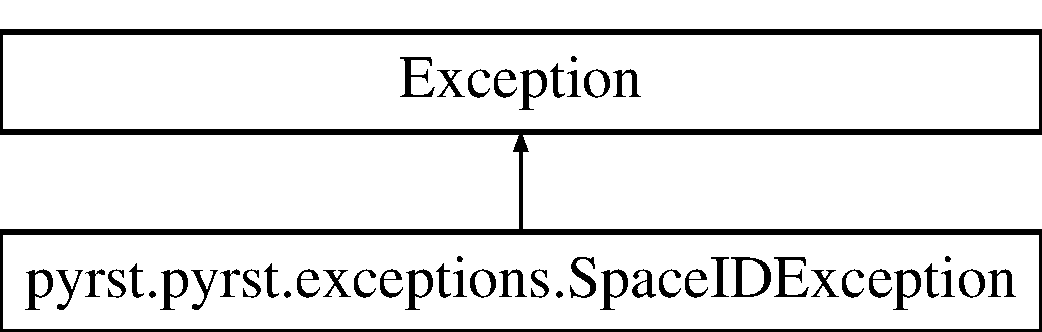
\includegraphics[height=2.000000cm]{classpyrst_1_1pyrst_1_1exceptions_1_1_space_i_d_exception}
\end{center}
\end{figure}
\subsection*{Public Member Functions}
\begin{DoxyCompactItemize}
\item 
\hypertarget{classpyrst_1_1pyrst_1_1exceptions_1_1_space_i_d_exception_a3fff28c3727c09e36c3c757989d175d3}{}def {\bfseries \+\_\+\+\_\+repr\+\_\+\+\_\+} (self)\label{classpyrst_1_1pyrst_1_1exceptions_1_1_space_i_d_exception_a3fff28c3727c09e36c3c757989d175d3}

\end{DoxyCompactItemize}


The documentation for this class was generated from the following file\+:\begin{DoxyCompactItemize}
\item 
pyrst/exceptions.\+py\end{DoxyCompactItemize}

\hypertarget{classpyrst_1_1pyrst_1_1exceptions_1_1_token_exception}{}\section{pyrst.\+pyrst.\+exceptions.\+Token\+Exception Class Reference}
\label{classpyrst_1_1pyrst_1_1exceptions_1_1_token_exception}\index{pyrst.\+pyrst.\+exceptions.\+Token\+Exception@{pyrst.\+pyrst.\+exceptions.\+Token\+Exception}}
Inheritance diagram for pyrst.\+pyrst.\+exceptions.\+Token\+Exception\+:\begin{figure}[H]
\begin{center}
\leavevmode
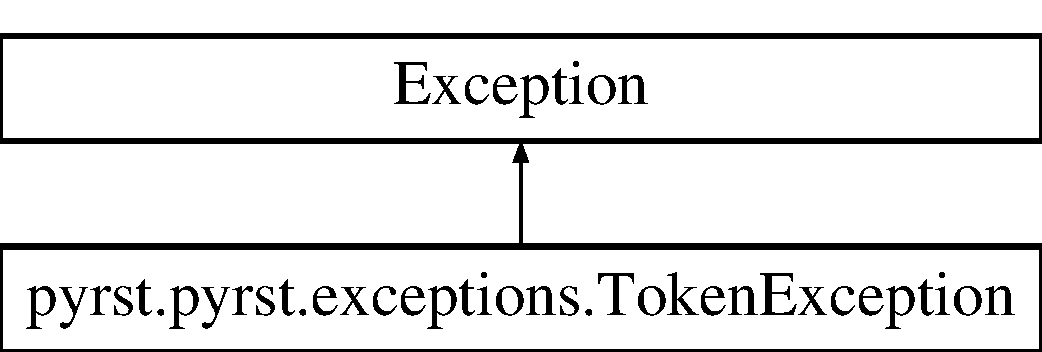
\includegraphics[height=2.000000cm]{classpyrst_1_1pyrst_1_1exceptions_1_1_token_exception}
\end{center}
\end{figure}
\subsection*{Public Member Functions}
\begin{DoxyCompactItemize}
\item 
\hypertarget{classpyrst_1_1pyrst_1_1exceptions_1_1_token_exception_a49b4f43747cd51fc89a65a5cbf41effd}{}def {\bfseries \+\_\+\+\_\+init\+\_\+\+\_\+} (self, value)\label{classpyrst_1_1pyrst_1_1exceptions_1_1_token_exception_a49b4f43747cd51fc89a65a5cbf41effd}

\item 
\hypertarget{classpyrst_1_1pyrst_1_1exceptions_1_1_token_exception_a27ddf6a9367becc47dd49120833b597b}{}def {\bfseries \+\_\+\+\_\+repr\+\_\+\+\_\+} (self)\label{classpyrst_1_1pyrst_1_1exceptions_1_1_token_exception_a27ddf6a9367becc47dd49120833b597b}

\end{DoxyCompactItemize}
\subsection*{Public Attributes}
\begin{DoxyCompactItemize}
\item 
\hypertarget{classpyrst_1_1pyrst_1_1exceptions_1_1_token_exception_a8d767bd65e335b8dd1fa3ac19df0768c}{}{\bfseries value}\label{classpyrst_1_1pyrst_1_1exceptions_1_1_token_exception_a8d767bd65e335b8dd1fa3ac19df0768c}

\end{DoxyCompactItemize}


The documentation for this class was generated from the following file\+:\begin{DoxyCompactItemize}
\item 
pyrst/exceptions.\+py\end{DoxyCompactItemize}

%--- End generated contents ---

% Index
\backmatter
\newpage
\phantomsection
\clearemptydoublepage
\addcontentsline{toc}{chapter}{Index}
\printindex

\end{document}
